\documentclass[usenames,dvipsnames, aspectratio=169, 9pt]{beamer}
\beamertemplatenavigationsymbolsempty
\setbeamertemplate{footline}[frame number]
\setbeamertemplate{section in toc}[sections numbered]
\usecolortheme[named=Plum]{structure}
\usefonttheme{serif}
\usepackage{amsmath, amsthm, amssymb, pgffor, multirow, booktabs, tabularx, multirow, graphicx, pgffor, arydshln}
\usepackage{kotex}
\usepackage{epstopdf}
\usepackage{grffile}


\author{Boyeon Kim}
\institute{Department of Mathematics, School of Mathematics and Computing \\ Mathematics \\ Yonsei University}
\date{January 6, 2023}
\title{Comparison : DQN vs. Adjoint Method on Optimal control}

\def\bs{\boldsymbol}
\usepackage{grffile}
\begin{document}

  \maketitle
\begin{frame}{SLIAR Optimal control}
    \begin{itemize}
        \item GAOL : SLIAR Model optimal control
        \item Method 1 : Adjoint Method
        \item Method 2 : DQN
    \end{itemize}
\end{frame}


\begin{frame}\frametitle{SLIAR Model}
    \begin{itemize}
        \item SLIAR Model Equations and structure.
    \end{itemize}
    $\begin{cases}
        S' &= -\beta (1-\sigma) S\Lambda - \nu S\\
        L' &= \beta (1-\sigma) S\Lambda - \kappa L\\
        I' &= p\kappa L - \alpha I - \tau I \\
        A' &= (1-p)\kappa L - \eta A \\
   \end{cases}$ \qquad with $\Lambda = \epsilon L + (1 - q) I + \delta A$
    \centering
    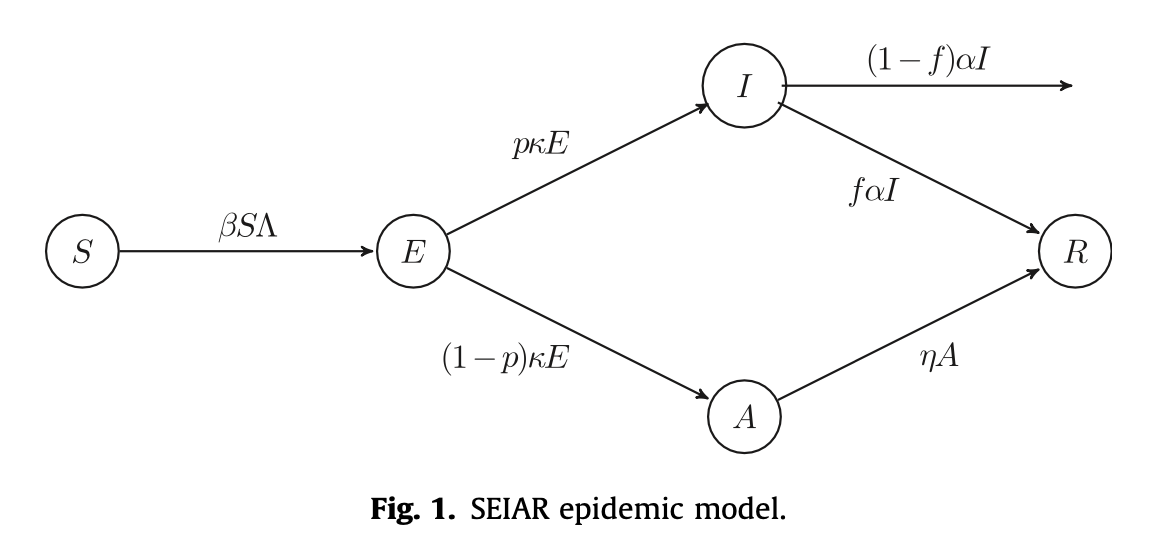
\includegraphics[width=10cm]{figure/sliar_diag.png}
\end{frame}


\begin{frame}\frametitle{SLIAR model parameters}
    \centering
    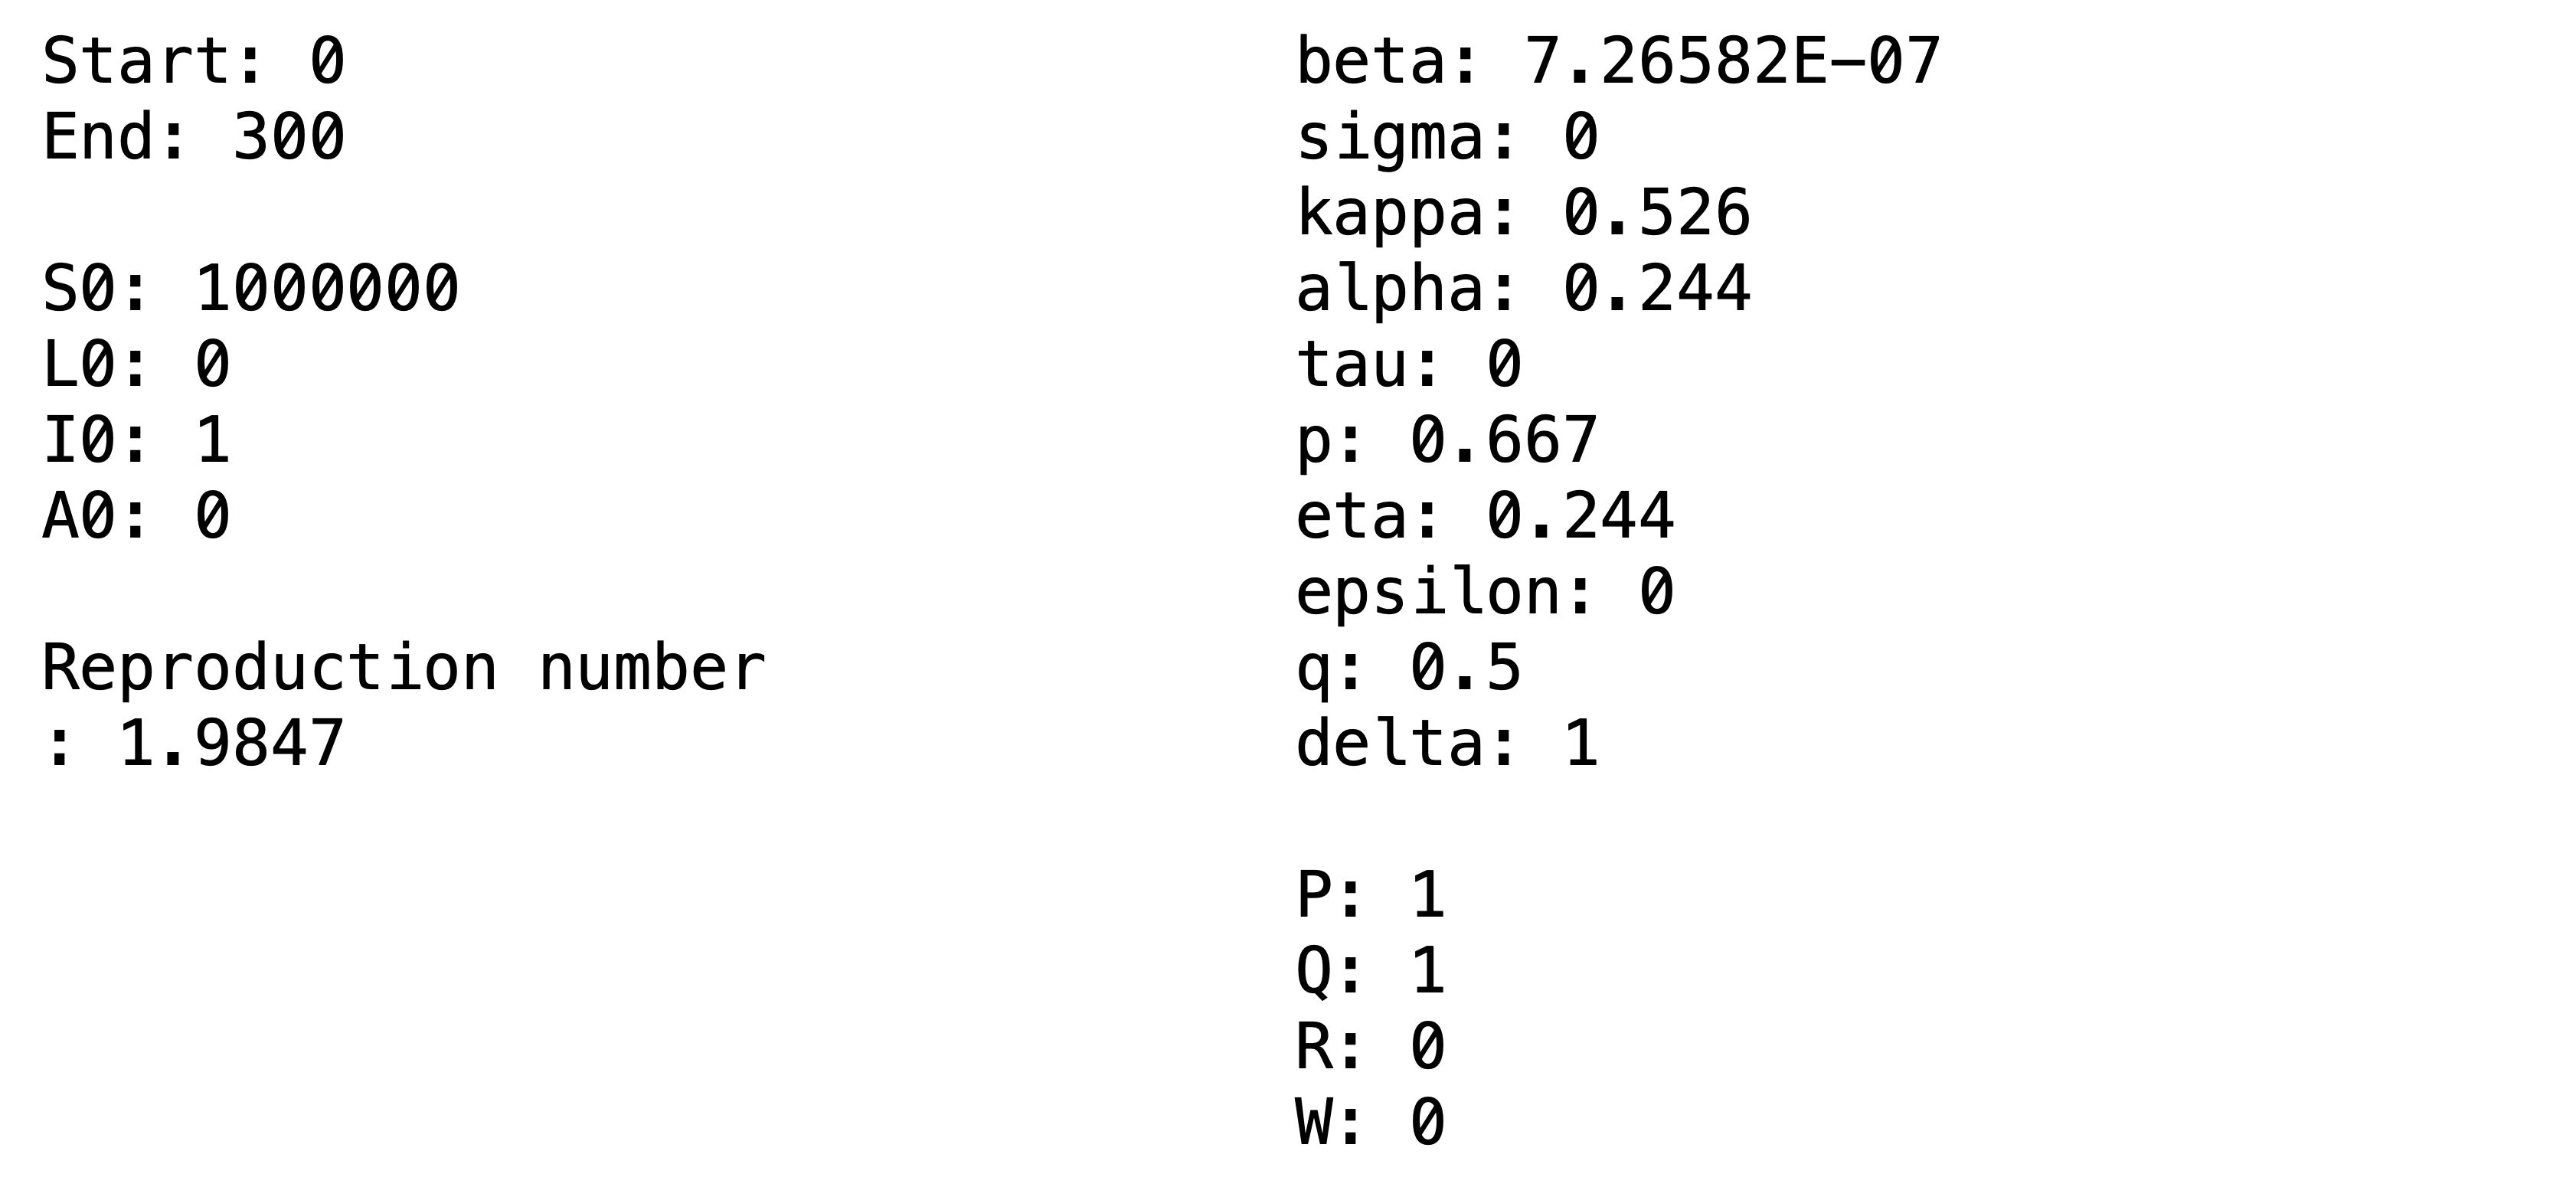
\includegraphics[width=10cm]{figure/sliar_parameter.png}
\end{frame}


\begin{frame}\frametitle{SLIAR w/o constrol}
    \centering
    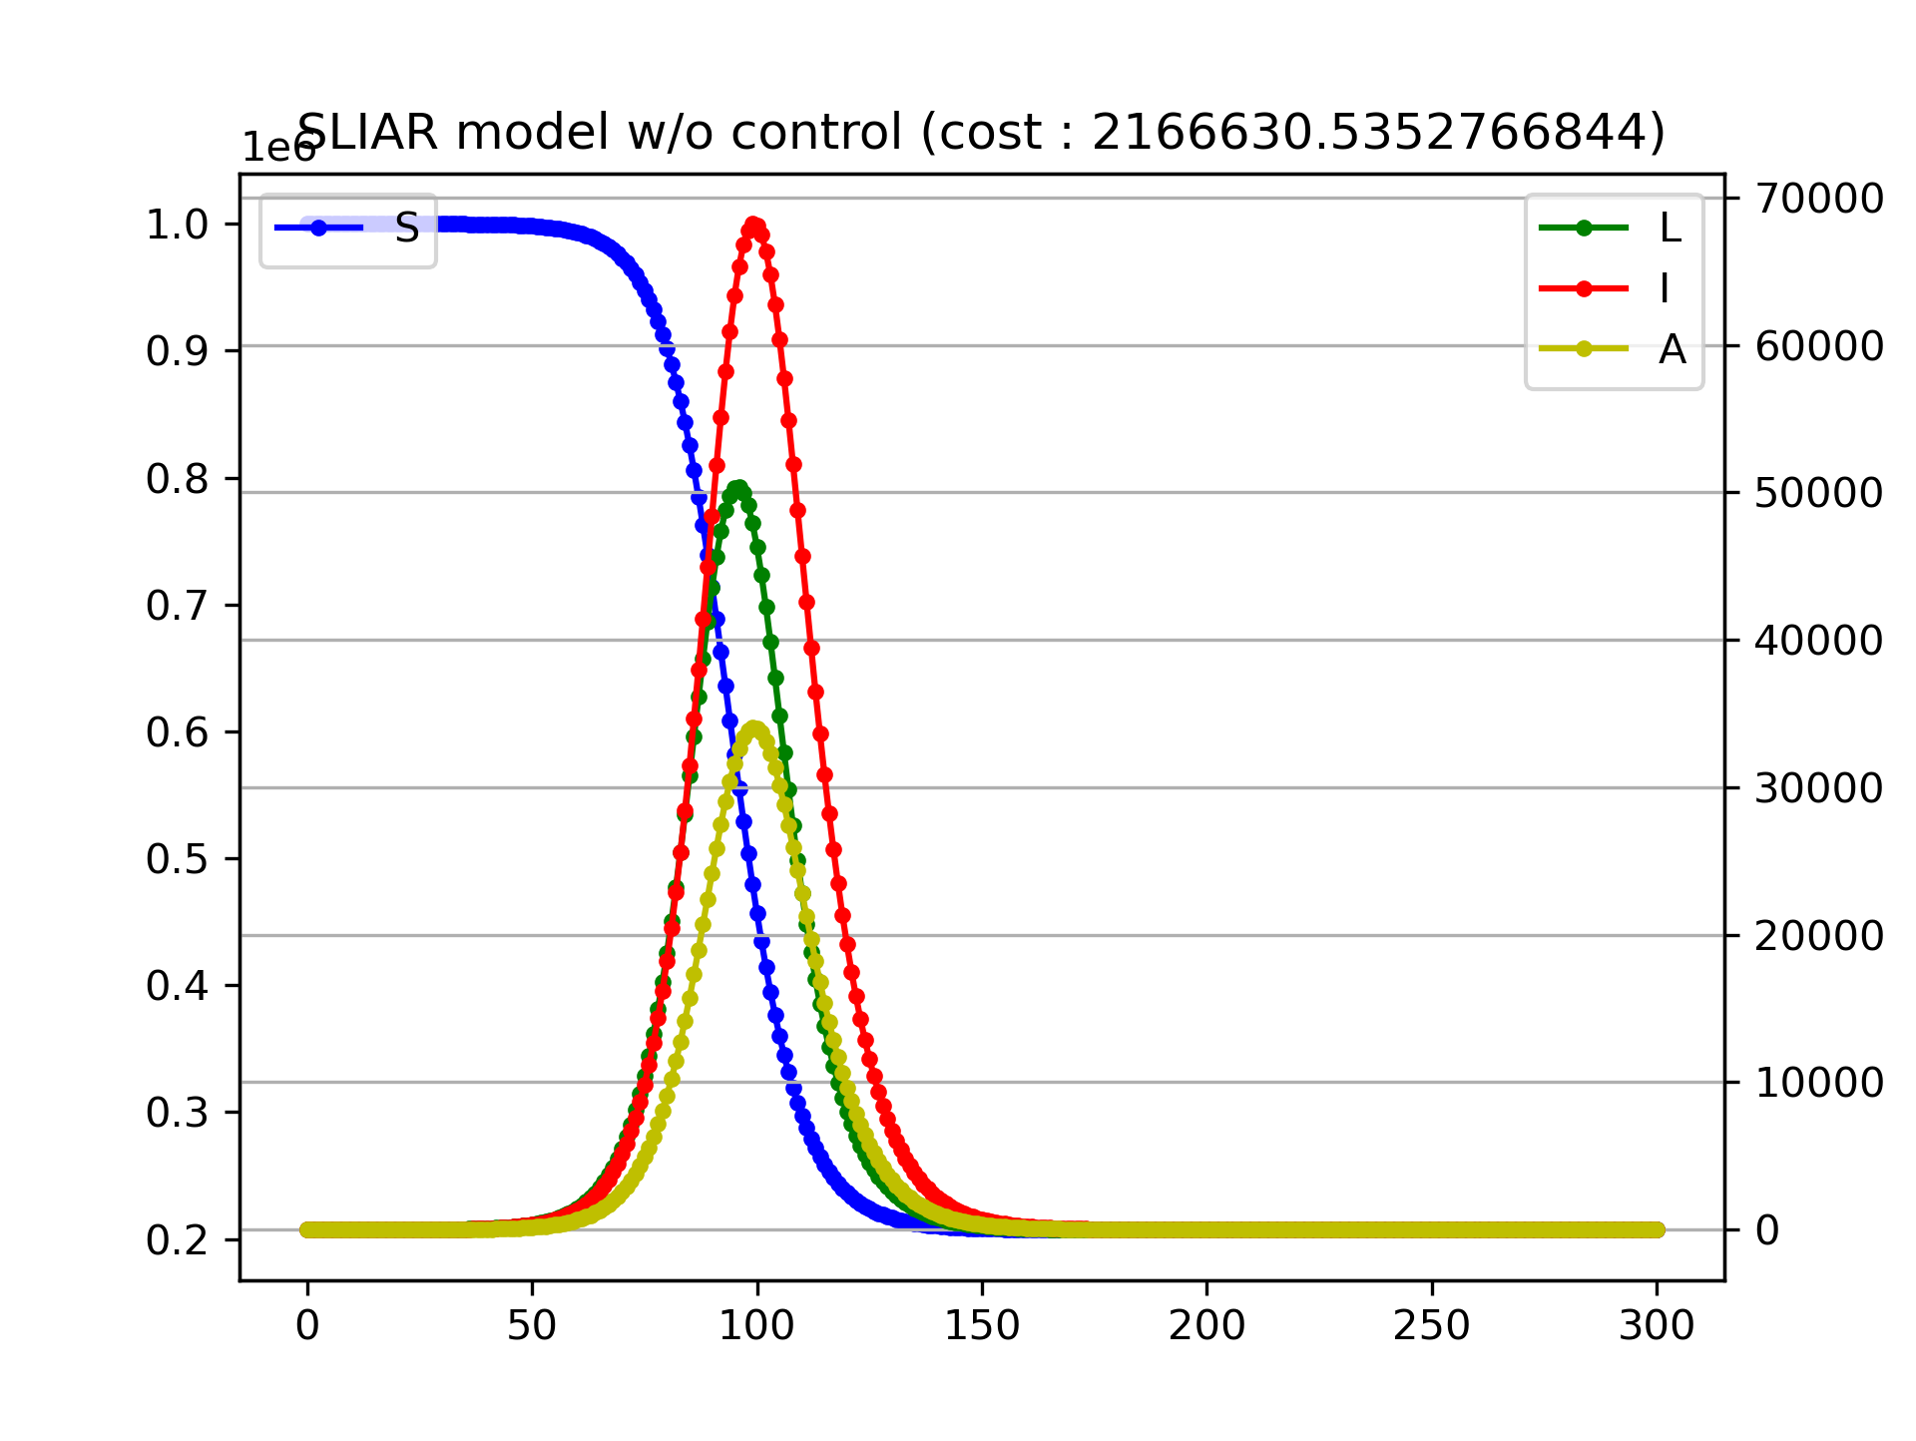
\includegraphics[width=10cm]{figure/sliar_wo_control.png}
\end{frame}


\begin{frame}\frametitle{SLIAR optimal control}
\begin{align*}
\min_{u\in\mathcal{U}_{ad}} \int_0^T PI(t) + Q\nu^2(t) + R\tau^2(t) + W\sigma^2(t) dt
\end{align*}

    subject to 
    \begin{align*}
    \begin{cases}
        S' &= -\beta (1-\sigma) S\Lambda - \nu S\\
        L' &= \beta (1-\sigma) S\Lambda - \kappa L\\
        I' &= p\kappa L - \alpha I - \tau I \\
        A' &= (1-p)\kappa L - \eta A \\
   \end{cases} \qquad with \quad \Lambda = \epsilon L + (1 - q) I + \delta A
   \end{align*}
\end{frame}

\begin{frame}\frametitle{SLIAR optimal control}
\begin{itemize}
\item $ \min_{u\in\mathcal{U}_{ad}} \int_0^T PI(t) + Q\nu^2(t) + R\tau^2(t) + W\sigma^2(t) dt$
\item Method : DQN
\item P = 1, Q = 1, iteration : 10,000
\end{itemize}
    \centering
    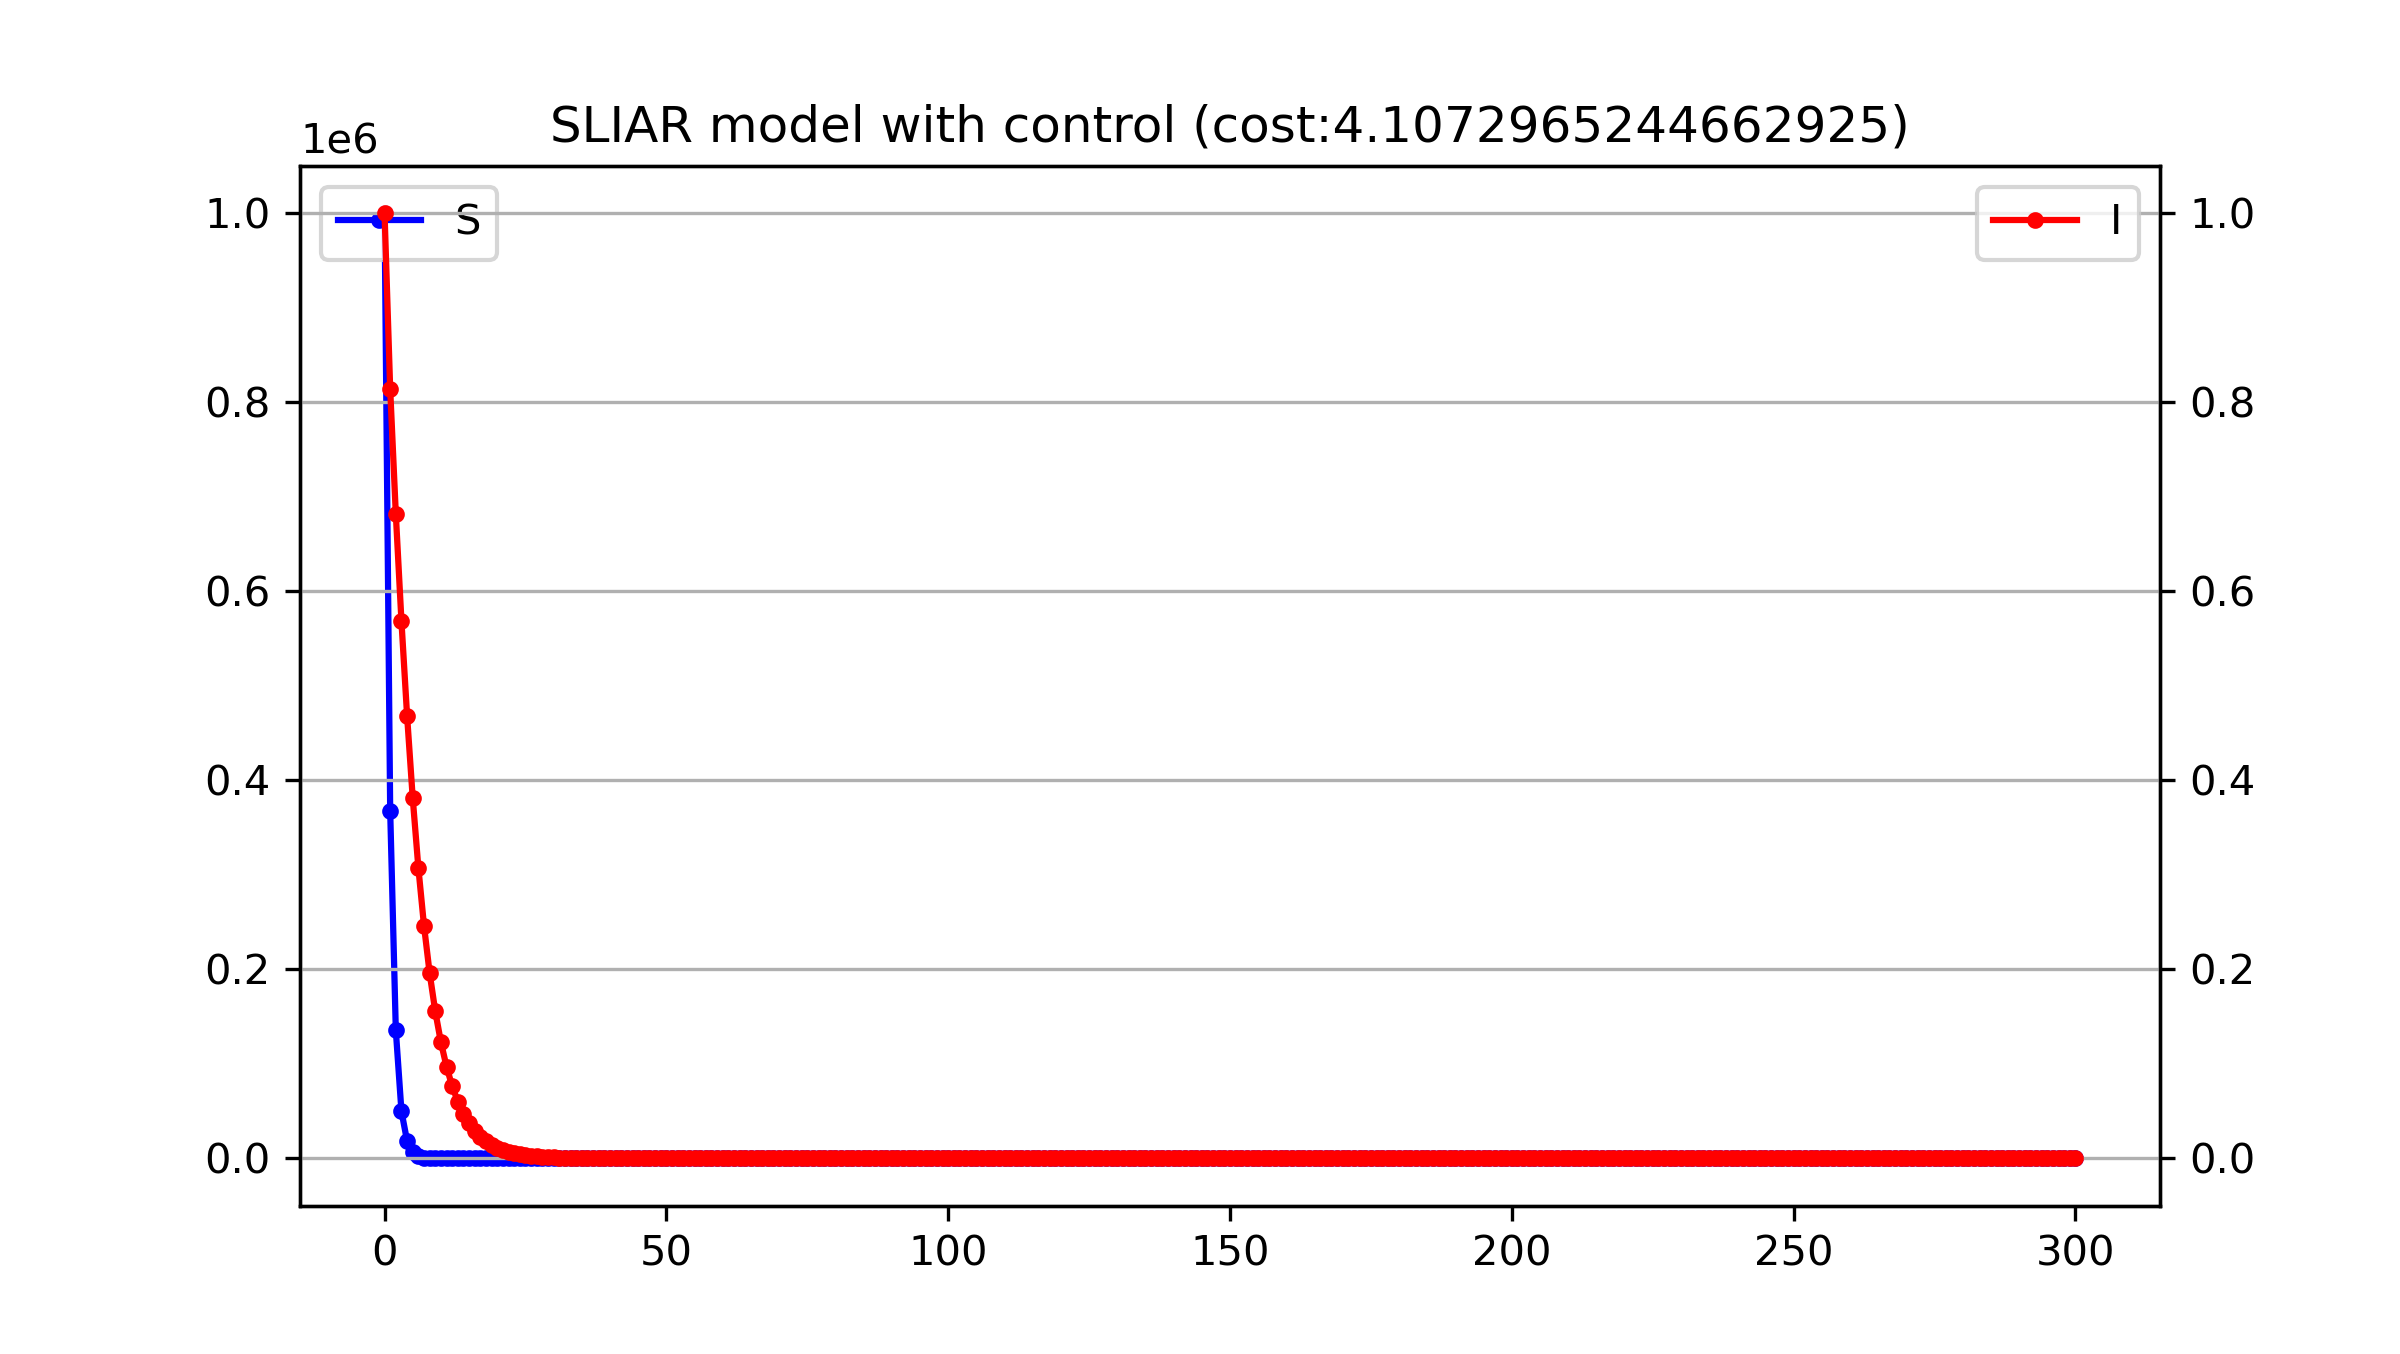
\includegraphics[width=6.5cm]{figure/sliar_dqn.png}
    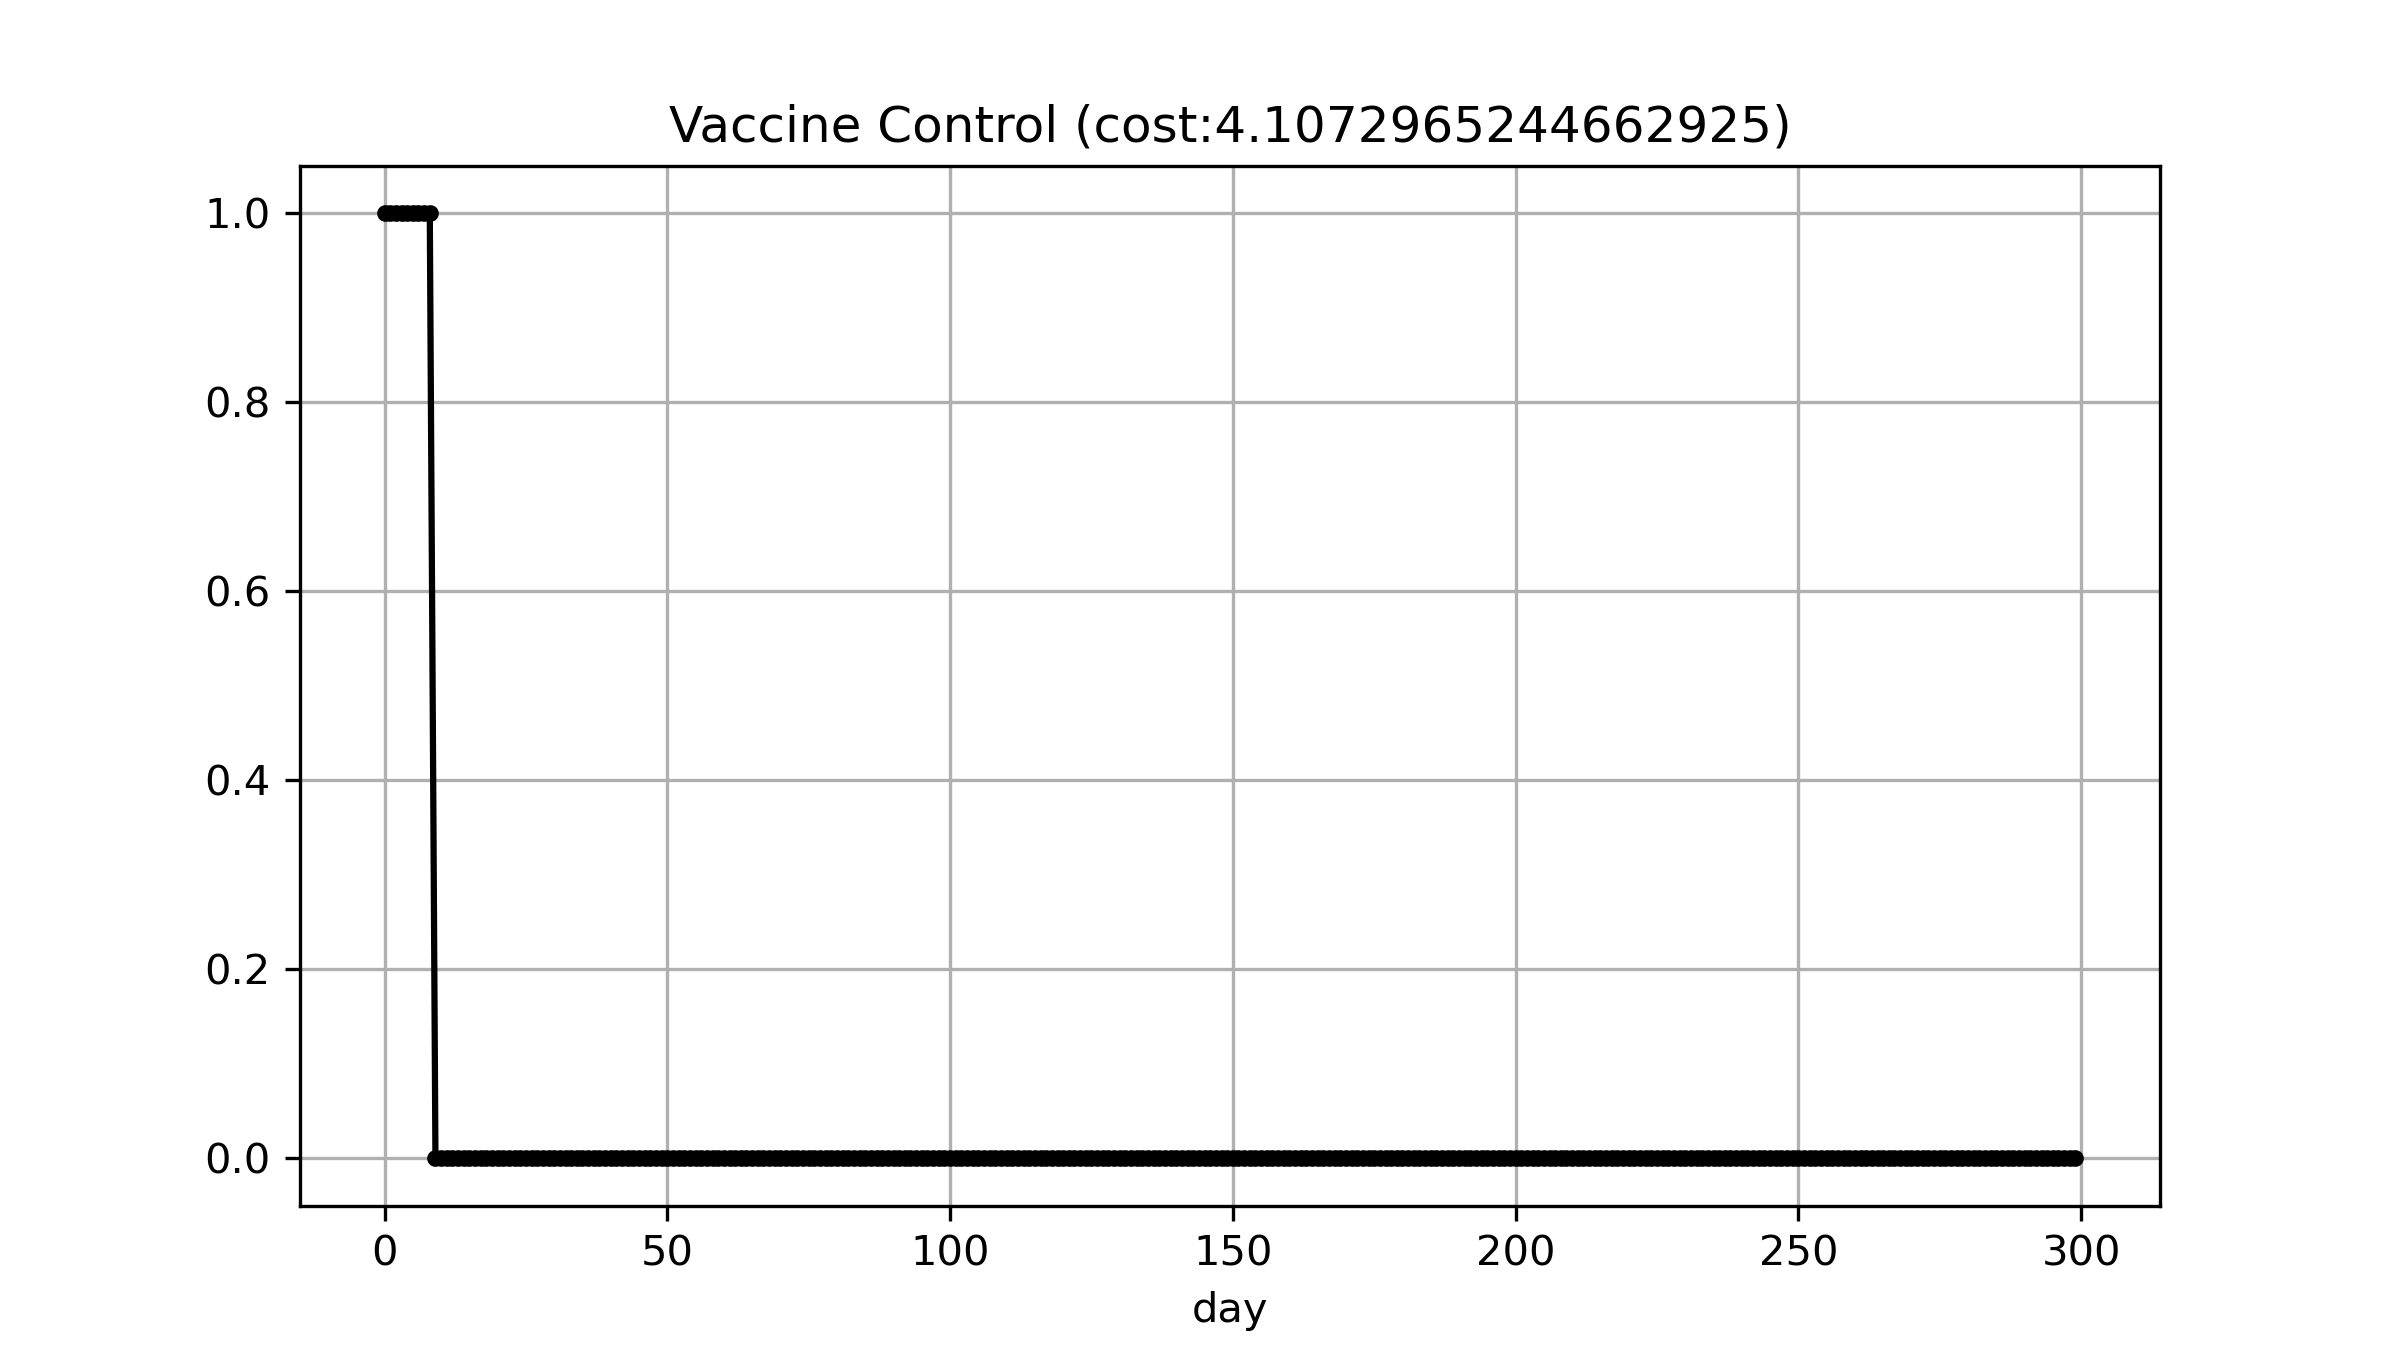
\includegraphics[width=6.5cm]{figure/sliar_dqn_control.png}
\end{frame}


\begin{frame}\frametitle{SLIAR optimal control}
\begin{itemize}
    \item Method : Adjoint Method
    \item Hamilonian
\end{itemize}

\begin{align*}
    H &= f + \lambda\cdot g\\
     &= PI + Q\nu^2 + R\tau^2 + W\sigma^2 + {\begin{bmatrix}\lambda_S\\\lambda_L\\\lambda_I\\\lambda_A\end{bmatrix}}' \cdot \begin{bmatrix}-\beta (1-\sigma) S\Lambda - \nu S\\ \beta (1-\sigma) S\Lambda - \kappa L\\ p\kappa L - \alpha I - \tau I \\ (1-p)\kappa L - \eta A \end{bmatrix}\\
     \lambda' &= -\frac{\partial H}{\partial x} 
\end{align*}
\end{frame}

\begin{frame}\frametitle{SLIAR optimal control}
\begin{itemize}
    \item Method : Adjoint Method
    \item Adjoint Equations
\end{itemize}
    $\begin{cases}
        \lambda_S' &= \nu \lambda_S + \beta (1- \sigma)\Lambda(\lambda_S - \lambda_L) \\
        \lambda_L' &= \beta (1- \sigma) \epsilon S (\lambda_S - \lambda_L)- \kappa p (\lambda_I - \lambda_A) + \kappa (\lambda_L - \lambda_A)\\
        \lambda_I' &= - P + \beta (1 - q) (1 - \sigma) S (\lambda_S - \lambda_L) + \lambda_I (\alpha + \tau)\\
        \lambda_A' &= \beta (1- \sigma) \delta S (\lambda_S - \lambda_L) +  \eta \lambda_A\\
    \end{cases}$
\end{frame}

\begin{frame}\frametitle{SLIAR optimal control}
\begin{itemize}
    \item Method : Adjoint Method
    \item Foward-Backward Sweep
\end{itemize}
    \centering
    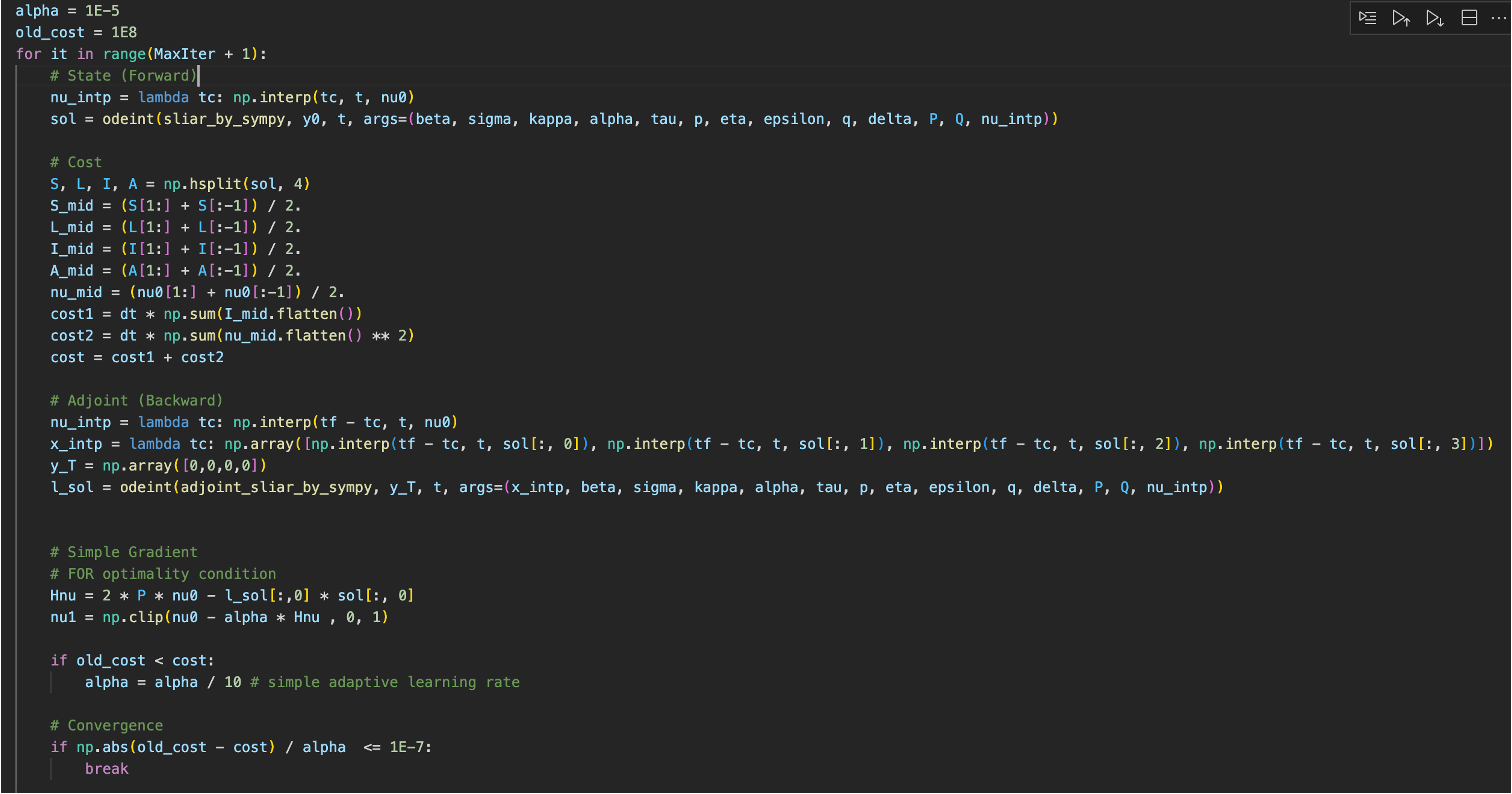
\includegraphics[width=10cm]{figure/code.png}
\end{frame}

\begin{frame}\frametitle{SLIAR optimal control}
\begin{itemize}
\item $ \min_{u\in\mathcal{U}_{ad}} \int_0^T PI(t) + Q\nu^2(t) + R\tau^2(t) + W\sigma^2(t) dt$
\item Method : Adjoint Method
\item P = 1, Q = 1
\end{itemize}
    \centering
    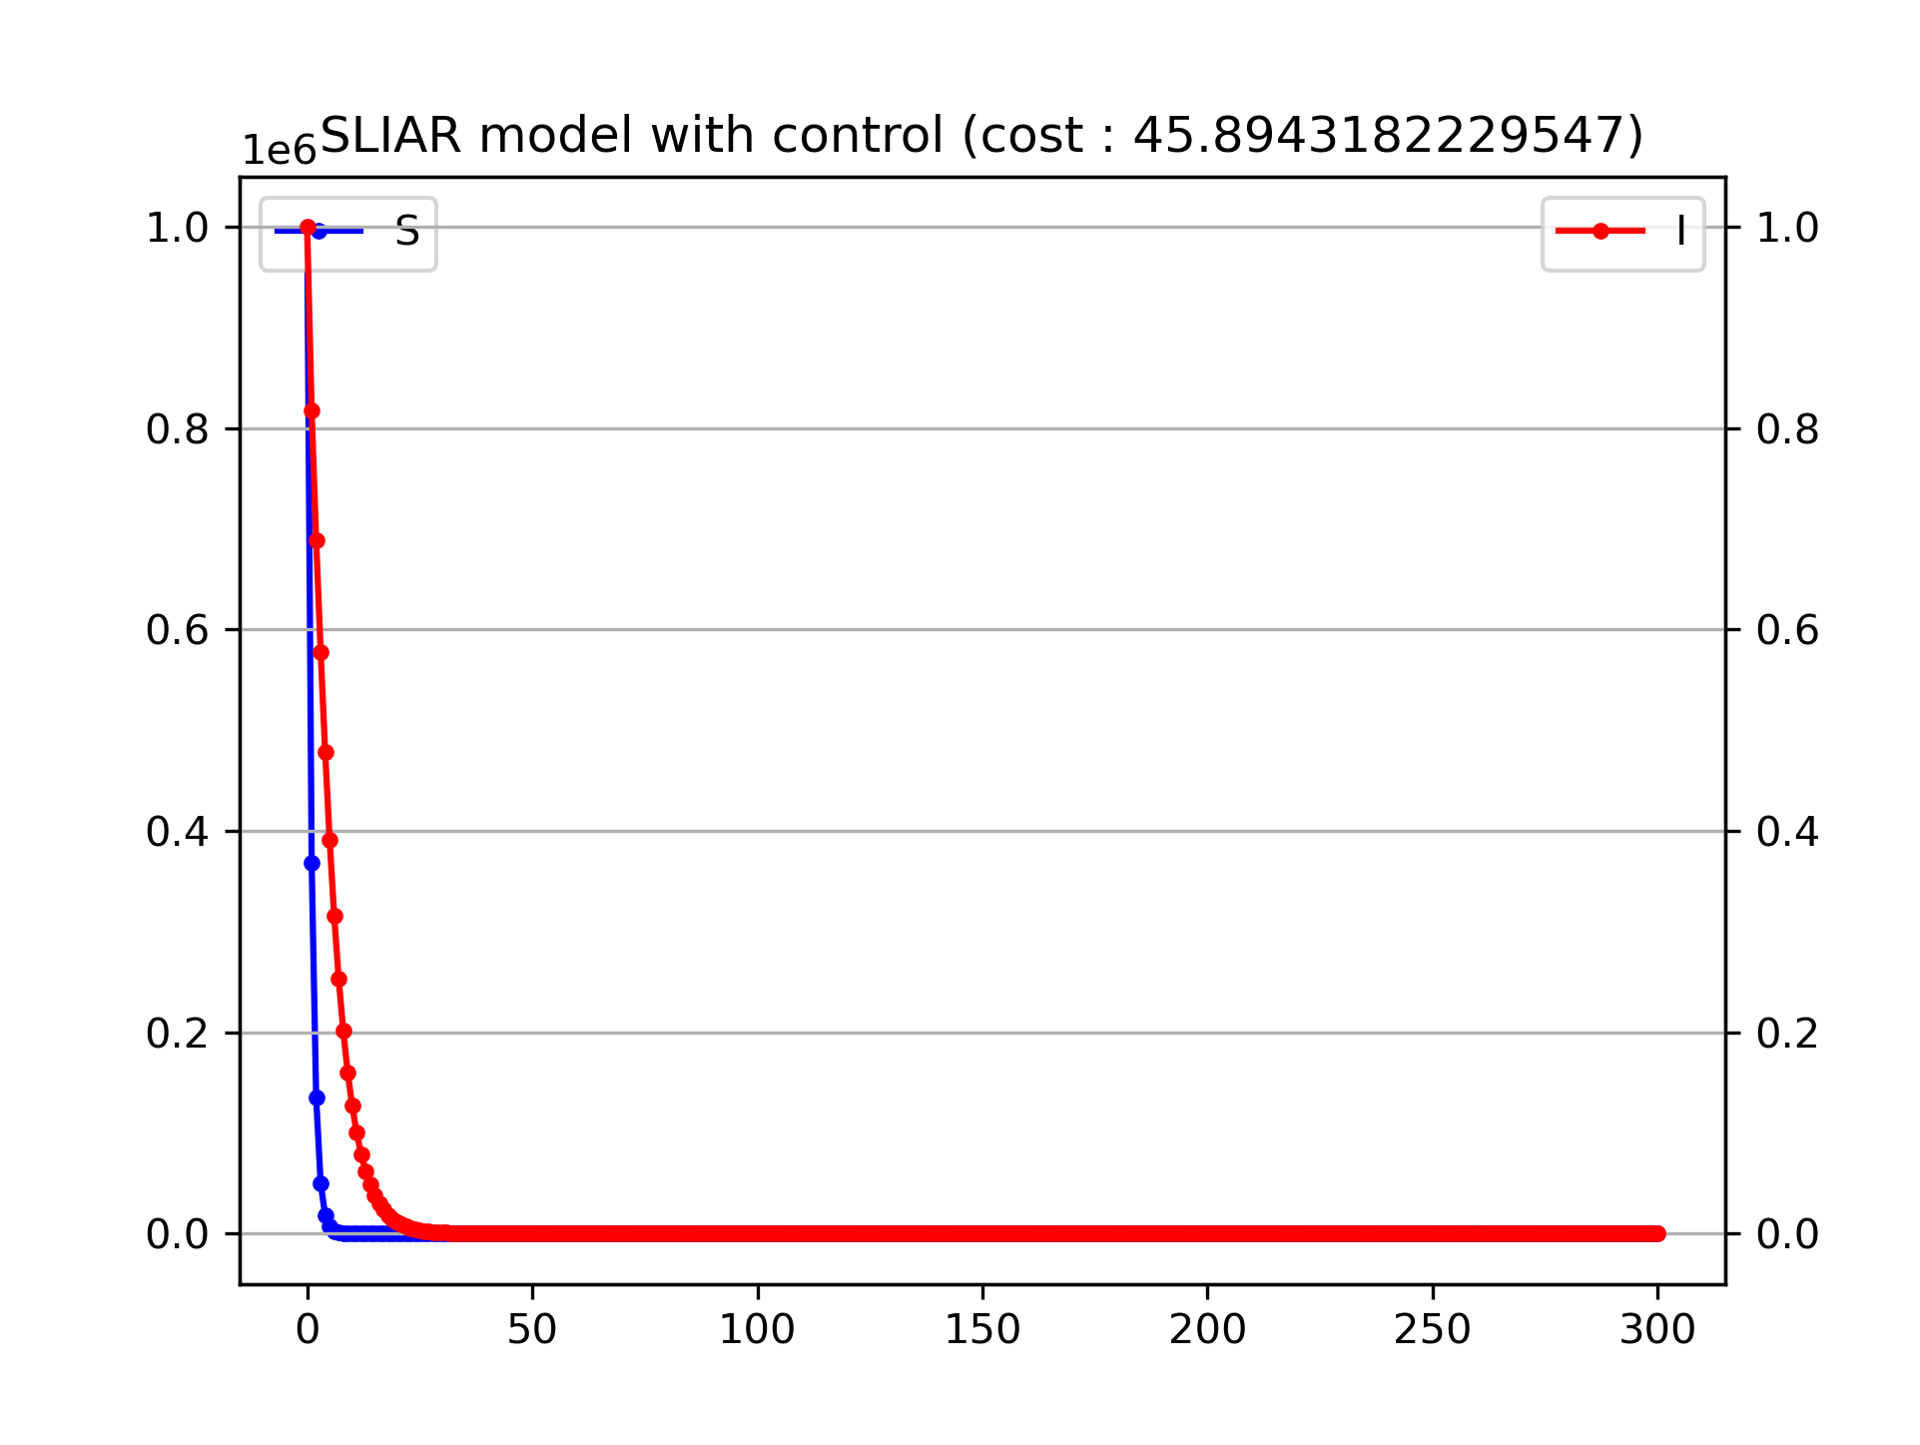
\includegraphics[width=6.5cm]{figure/sliar_adj.png}
    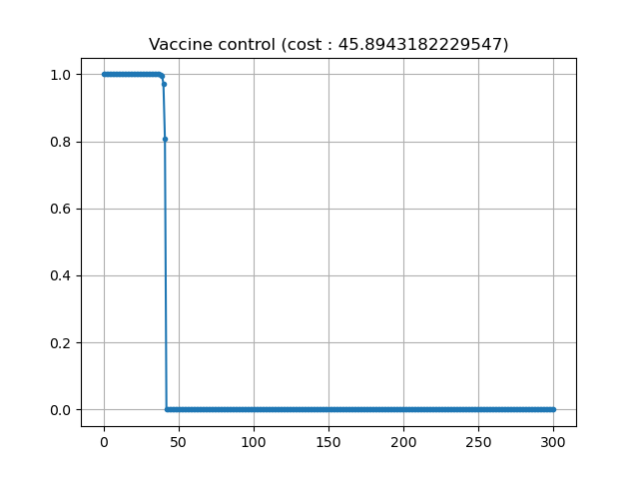
\includegraphics[width=6.5cm]{figure/sliar_adj_control.png}
\end{frame}

\begin{frame}\frametitle{Adjoint vs. DQN}
\begin{itemize}
\item $ \min_{u\in\mathcal{U}_{ad}} \int_0^T PI(t) + Q\nu^2(t) + R\tau^2(t) + W\sigma^2(t) dt$
\item Adjoint Method (left) vs. DQN (right)
\end{itemize}
    \centering
    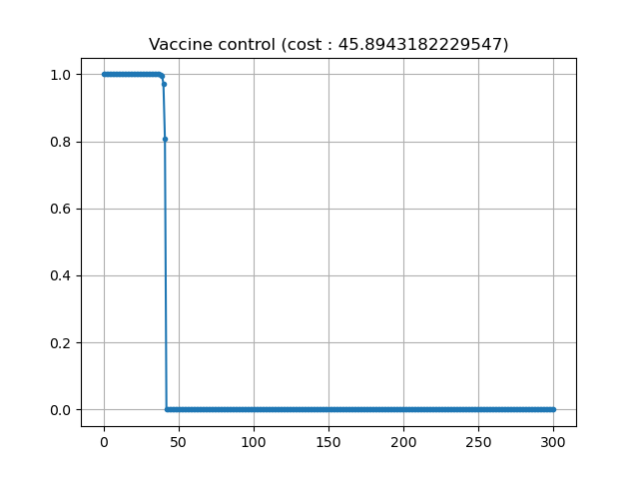
\includegraphics[width=6.5cm]{figure/sliar_adj_control.png}
    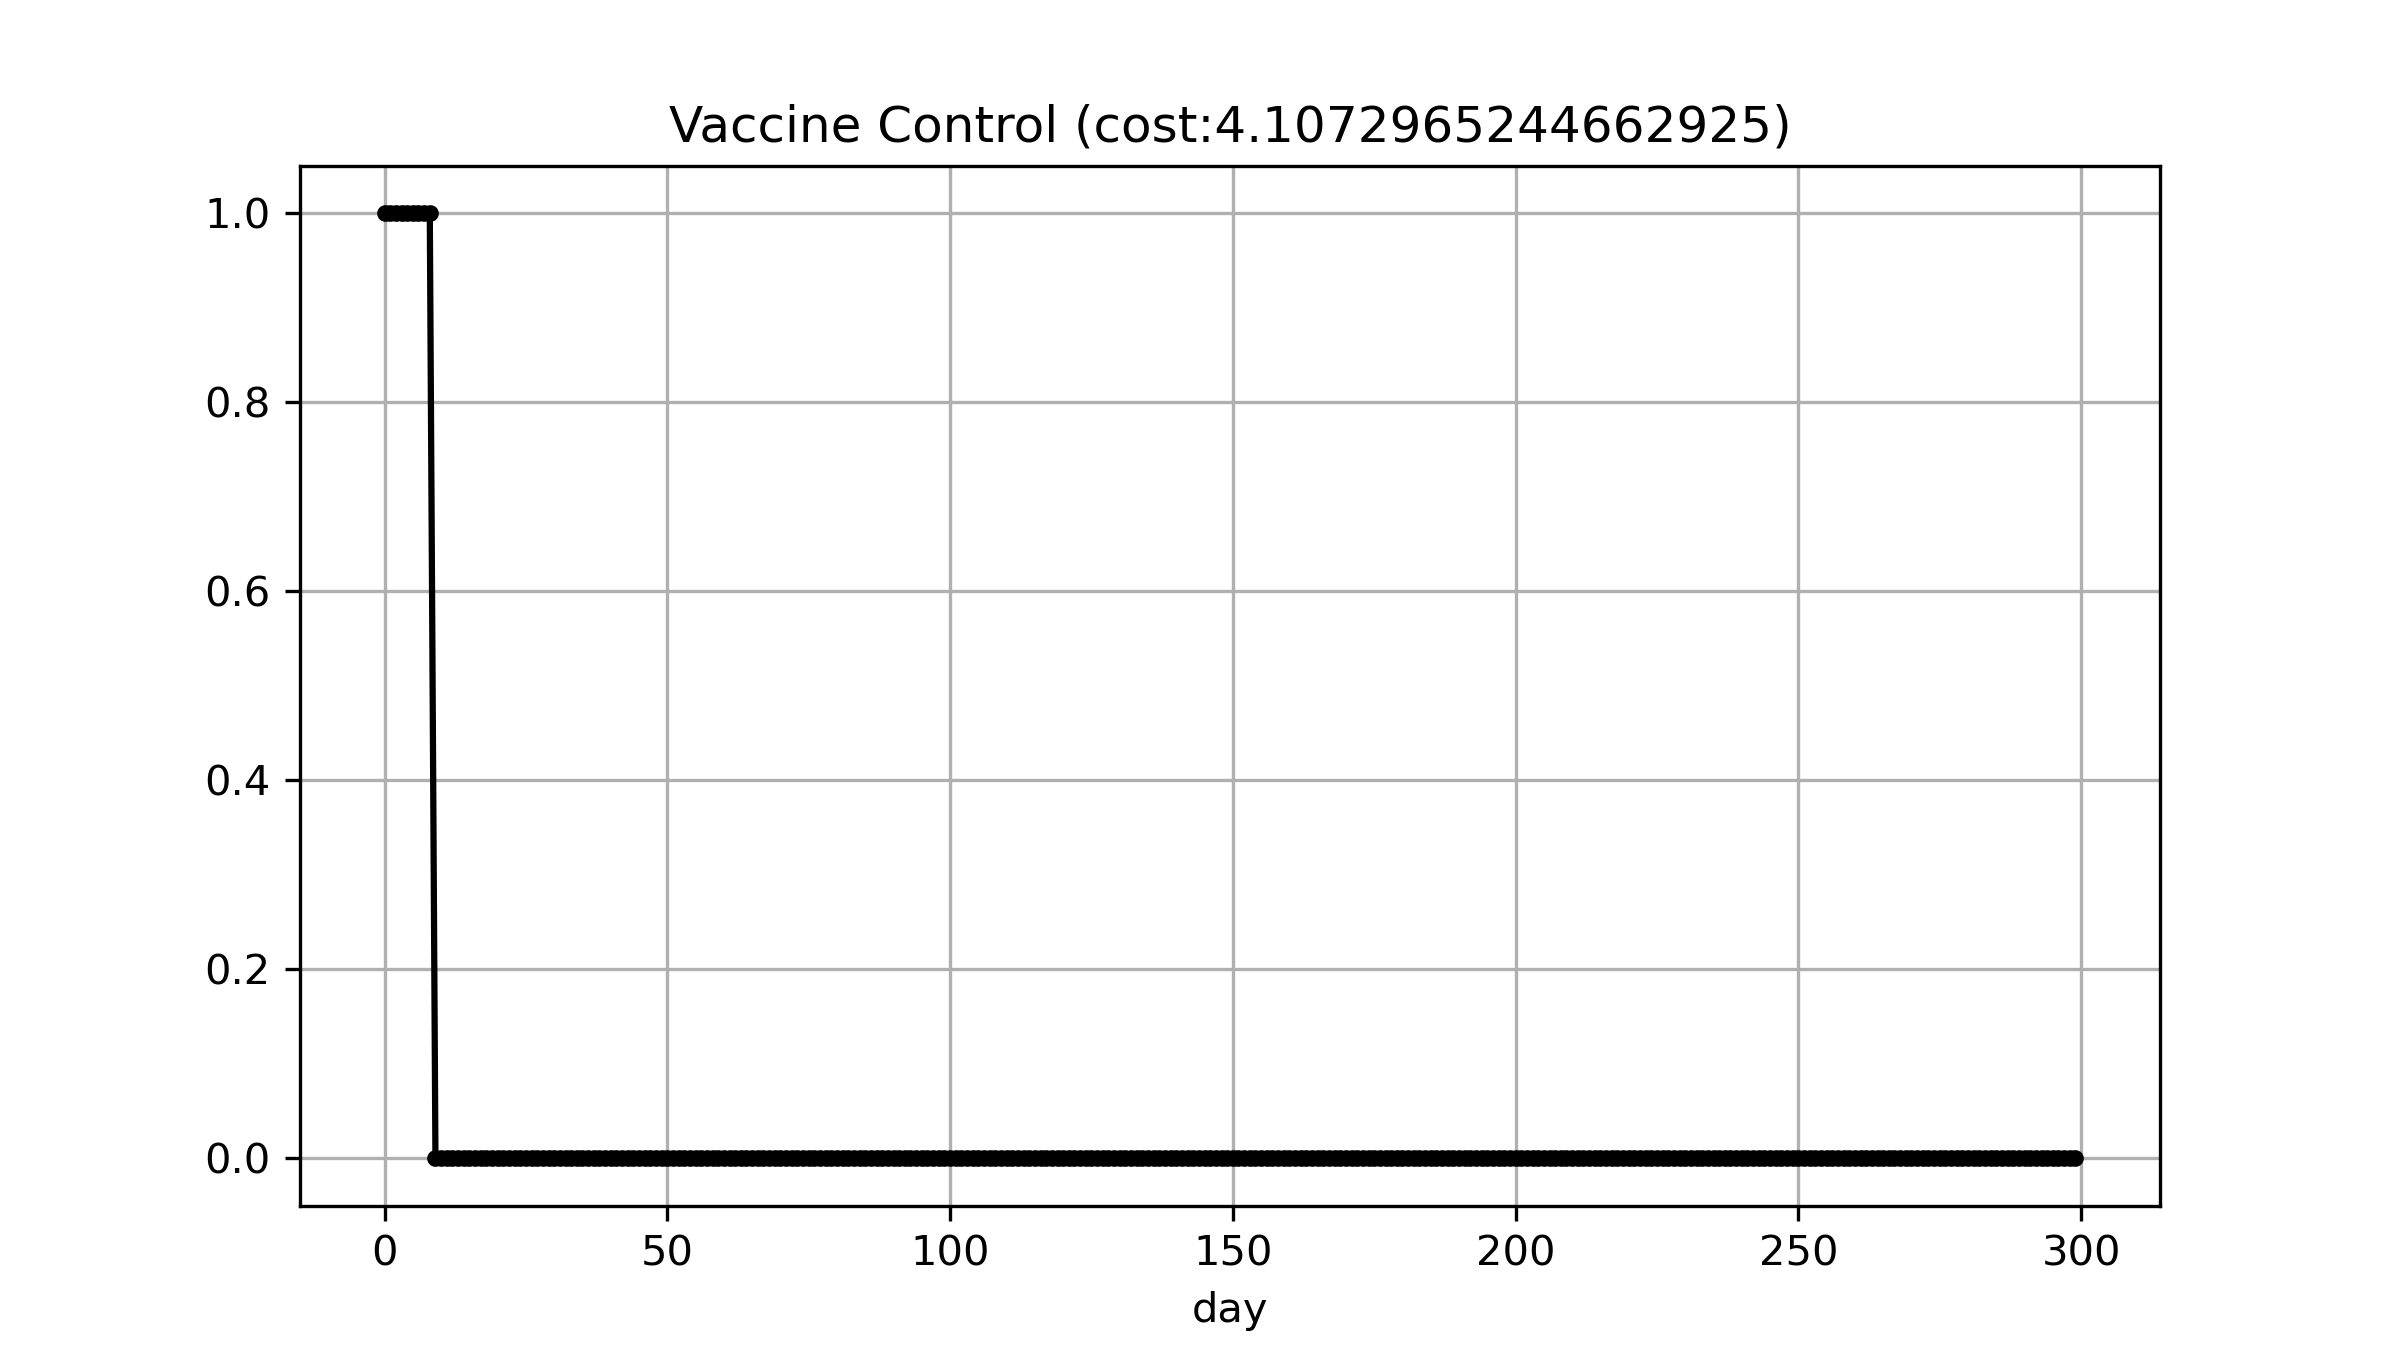
\includegraphics[height=4.1cm]{figure/sliar_dqn_control.png}
\end{frame}

\begin{frame}\frametitle{Another result of DQN}
\begin{itemize}
\item $ \min_{u\in\mathcal{U}_{ad}} \int_0^T PI(t) + Q\nu^2(t) + R\tau^2(t) + W\sigma^2(t) dt$
\item Method : DQN
\item P = 1, Q = 1e6, $\nu_max = 0.01$, iteration : 10,000
\end{itemize}
    \centering
    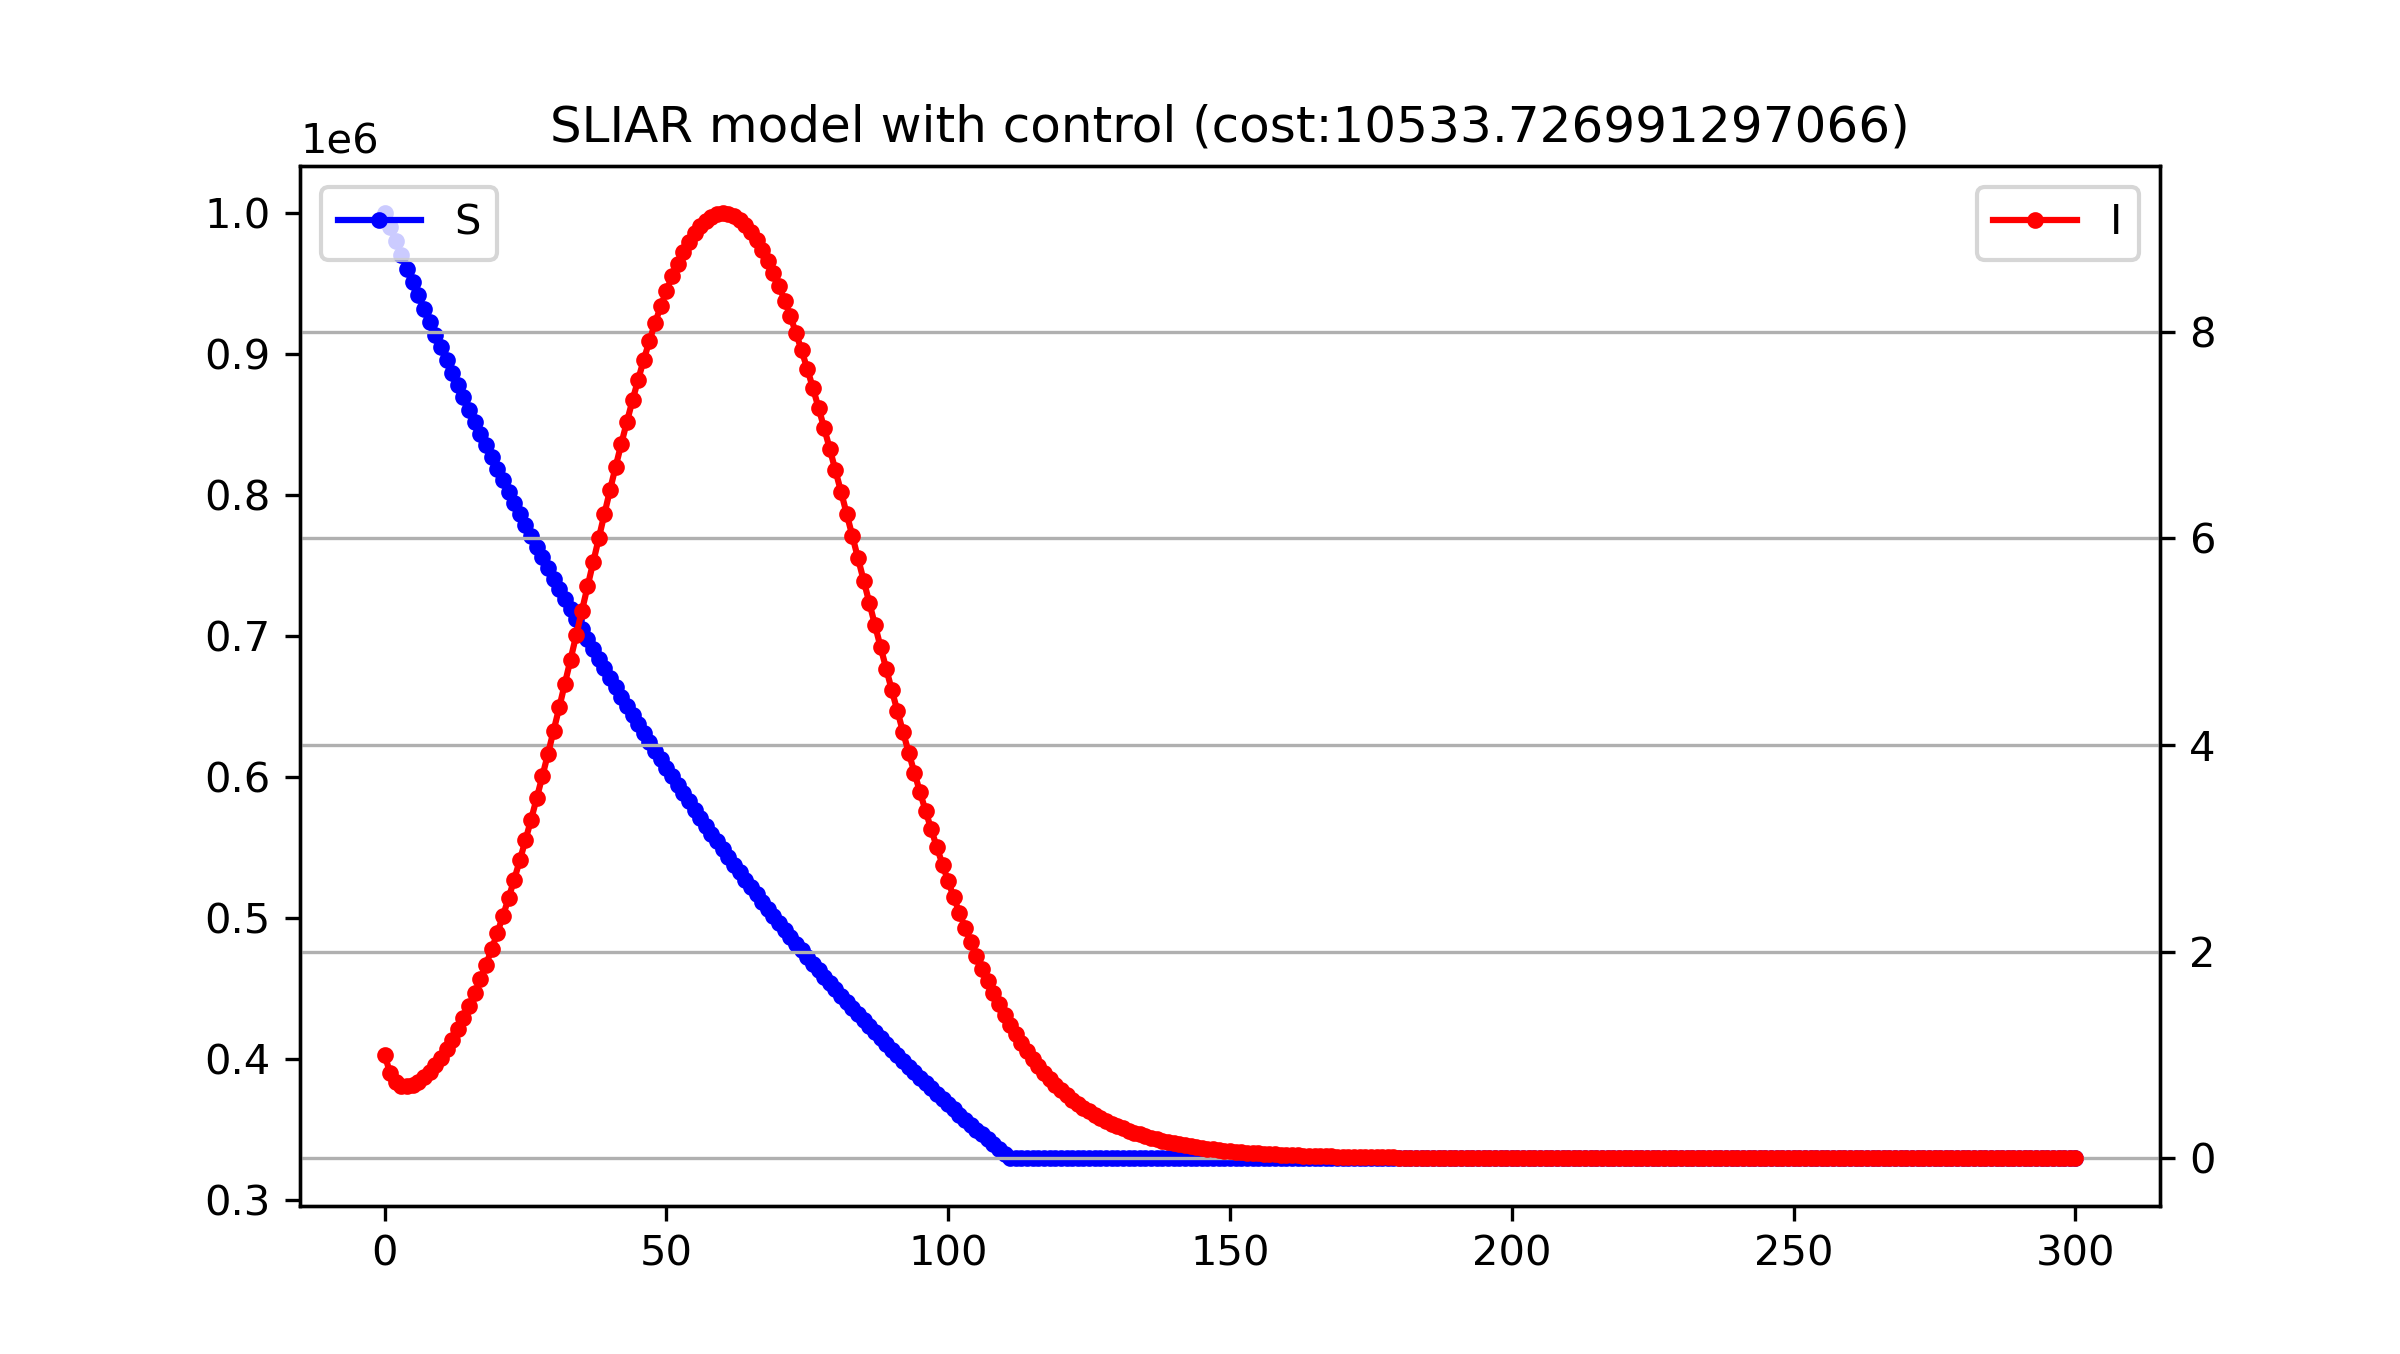
\includegraphics[width=6.5cm]{figure/sliar_dqn_numax.png}
    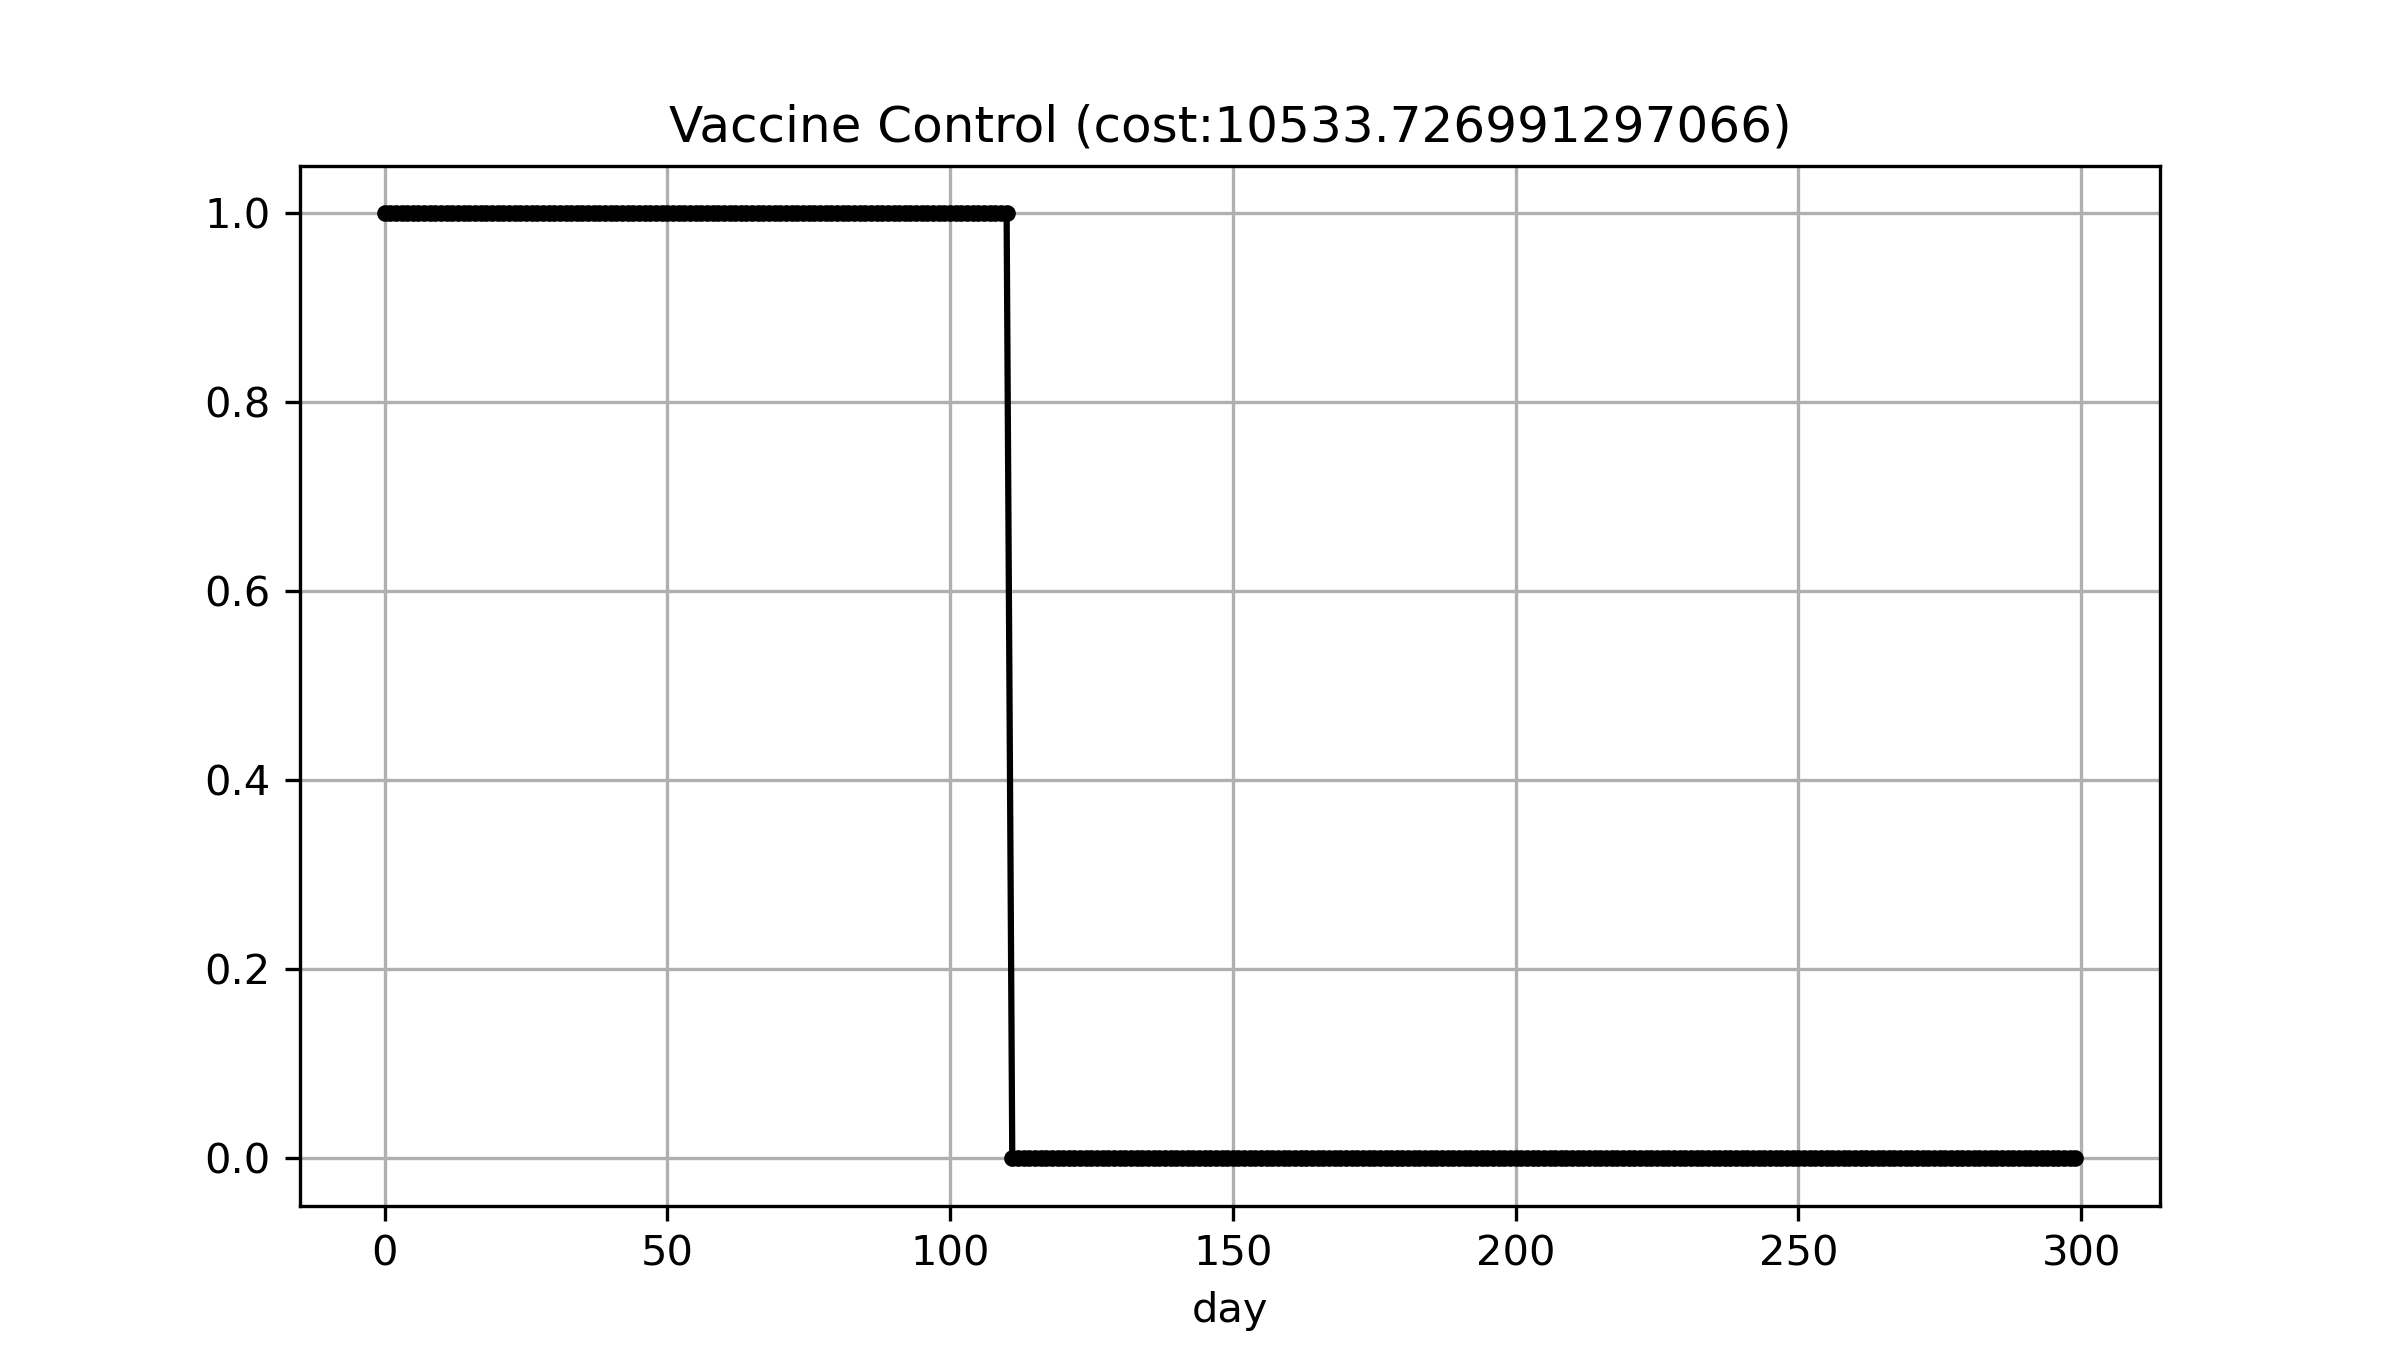
\includegraphics[width=6.5cm]{figure/sliar_dqn_numax_control.png}
\end{frame}

\begin{frame}\frametitle{Result of paper}
\begin{itemize}
\item $ \min_{u\in\mathcal{U}_{ad}} \int_0^T PI(t) + Q\nu^2(t) + R\tau^2(t) + W\sigma^2(t) dt$
\item Method : Adjoint Method
\item P = 1, Q = 1e6, $\nu_{max} = 0.01$
\end{itemize}
    \centering
    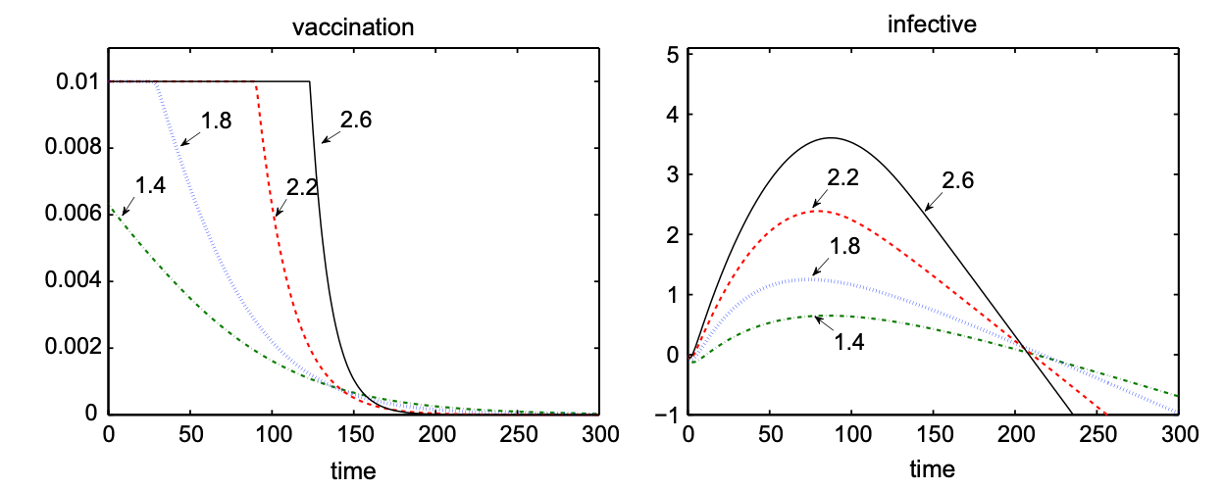
\includegraphics[width=10cm]{figure/result_paper_original.png}
\end{frame}

\begin{frame}\frametitle{Next todo list}
\begin{itemize}
\item Fix the adjoint method
\item Comparison : Adjoint method vs. DQN
\item Apply $\nu_{max} = 0.01$ to the adjoint method
\end{itemize}
\end{frame}

\end{document}